Os conjuntos que representam os conceitos são organizados em  módulos. Isso ocorre porque muitos conceitos apresentam similaridades, sendo razoável conceber uma taxonomia desses conjuntos organizando-os em conjuntos maiores. A Figura \ref{module} apresenta a estrutura de módulos (a fim de evitar poluição visual, as relações serão apresentadas em outra Figura). 

\begin{figure}[H]
  \centering
  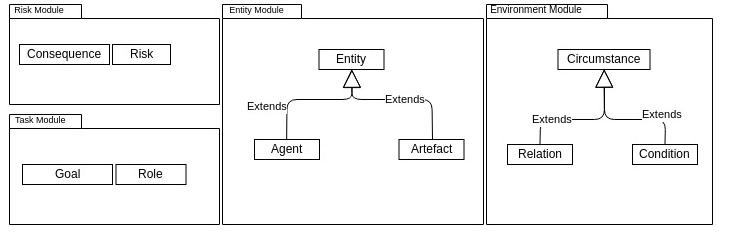
\includegraphics[width=1\linewidth]{figure/Module.jpeg} 
  \caption{A estrutura geral das classes do modelo}
  \label{module}
\end{figure}

Assim sendo, assumindo que existe $\Omega_{Model}$ (um conjunto global onde todos os outros conjuntos do modelo estão contidos nele), os módulos são representados da seguinte maneira: 

\begin{equation} 
    \Omega_{Model} = \{ M_{Risk}, M_{Task}, M_{Entity}, M_{Environment}\}
\end{equation}
\label{modules}


O mundo que este modelo pretende representar trabalha com o fato de que tanto agentes como artefatos possuem algumas propriedades em comum, que é: existem, ocupam lugar no espaço, estão sujeitos ao tempo, apresentam estados e participam de processos. Essa premissa possui os seus fundamentos alicerçados na \ref{agent} e \ref{artefact} e será demonstrado com maior rigor no texto que se segue. Tendo em vista a ocorrência de certos conceitos necessários para lidar com essas questões, se fez necessário definir um módulo de entidades para agrupa-los em uma estrutura única. Esse módulo é composto pelos seguintes conceitos:

\begin{equation} 
M_{Entity} = \{ Entity \}
\end{equation}\label{modent}

\textbf{Entity} - o termo entidade é sujeito a profundos debates filosóficos, porém neste texto o termo é usado para referenciar uma ``coisa'' que pode ser identificada, como uma pessoa, companhia ou um evento \cite{entity}. É de conhecimento que as propriedades anteriormente mencionadas caracterizam as ``coisas'' que podem ser identificadas, logo são entidades. É digno de nota a existência de entidades que não se adequam a todas essas propriedades. Contudo, essas propriedades fazem referência ao que se caracteriza por entidade, respeitando o conceito padrão \cite{entity} e restringindo para o escopo deste modelo. Isso contempla tanto os agentes como os artefatos, como fica claro na Relação \ref{defineentity}. O texto a seguir demonstra como essas propriedades se aplicam a agentes e a artefatos (sendo isso demonstrado, logo demonstrado-se que são entidades).

\textit{Ocupa lugar no espaço, estão sujeitos ao tempo - } como definido em \ref{agent} e \ref{artefact}, ambos são situados em ambientes. 
Isso possibilita inferir que se faça necessário a presença de um conceito que se apresente como uma propriedade de estado para agentes e artefatos. Um ambiente, no contexto onde os agentes e artefatos são usados para representar atividades das pessoas, condiz com a relação de espaço e tempo. 

\textit{Participa de Processos -} processos podem constituir entidades, bem como entidades necessariamente constituem processos por intermédio da ação que aquelas manifestam nesses. No que se verifica ao primeiro caso, é possível usar o ser humano como exemplo - onde
a entidade ser humano é formulada por uma série de processos bio-químicos. Sobre o segundo caso, relações climáticas exemplificam isso, onde a água é uma entidade presente em processos termodinâmicos. 

\textit{Apresenta estados -} o fato de que artefatos bem como agentes apresentam atributos (que podem mudar e podem assumir diferentes valores no que tange aos eventos externos e internos), então ambos também apresentam a concepção de estados (sendo esse termo usado diretamente em certos pontos dos textos presentes tanto em \ref{agent} \ref{artefact}). 


\begin{equation} \label{defineentity} 
 \{ Agent \cup Artefact \} \subset Entity
\end{equation}

\textbf{Agent} - esse estudo adota a definição de agentes presentes no primeiro parágrafo da Seção \ref{agent}. Isso implica em entidades autônomas, ou seja, que apresenta a capacidade de agir por si mesma quando diante de condições onde isso é necessário. A seção \ref{agent}, apresenta o conceito de agentes inteligentes e esse mesmo conceito é adotado neste modelo. 

Não é preocupação deste estudo, delimitar as representações do agente, bem como definir algoritmos para verificar como se dão às relações de tomada de decisão dos mesmos. Assim sendo, fica em aberto para o modelador definir como acontece os processos de tomada de decisão, estados internos e modelos de representação que serão usados para definir o comportando do agente. 

\textbf{Artefact} - são entidades que existem para que os agentes possam cumprir com os seus objetivos e que apresentam interface de uso, instruções de operação, funcionalidade e estrutura-comportamento. Essas entidades não são orientados à objetivos e 
não apresentam capacidade de comunicação como definido na Seção \ref{artefact}. Predicados que contemplam esses aspectos do artefato serão apresentados mais adiante ao decorrer do texto. 

Os agentes são autônomos e orientados à objetivos sendo esses dois elementos descaracterizantes do que se define por artefato. Logo, apesar de agentes e artefatos serem entidades, não é possível existir um agente que seja artefato ou um artefato que seja agente, o que é dado pela relação presente na Expressão \ref{agentsartefactvoid}. 

\begin{equation} \label{agentsartefactvoid}
    Agent \cap Artefact = \{ \emptyset \}
\end{equation}

Para tornar a apresentação de certos conceitos mais didática, o autor desenvolveu um exemplo entitulado por: \textbf{Exemplo da Redação}, que é o seguinte cenário: ``O Professor Aristóteles definiu uma atividade: escrever uma redação sobre o livro Metafísica. Para isso, o aluno Alexandre o Grande deve escrever um texto, deve ler o livro sobre o tópico em definido, deve pegar uma folha, deve pegar um lápis e escrever a redação''.  


\textbf{O Módulo de Atividades} - \textit{Task Module} representado por $M_{Task}$ condiz com os conceitos relacionados aos objetivos que devem ser atingidos, bem como aos papéis que são assumidos pelos agentes.
\begin{equation}
    M_{Task} = \{ Goal, Role \}
\end{equation}

\textbf{Goal} - faz referência aos objetivos que devem ser atingidos pelos agentes. Os fundamentos semânticos deste conjunto estão presentes na Seção \ref{sma} mais especificamente na subseção \ref{moiseformalizesma}. Neste modelo, um objetivo é descrito em termos de entidades relações e condições necessárias para que uma data atividade possa ser dada como concluída. 

\textbf{Role} - apresenta o papel que um agente pode adotar dentro de um \textit{SMA}. Esse conceito também é importado no \textit{MOISE+} 
\ref{moiseformalizesma} e define as relações deonticas entre os agentes e os objetivos. Para exemplificar, pode-se considerar o \textbf{Exemplo da Redação} onde existem dois agentes $Agent = \{ aristoteles, alexandre \}$, existem dois papéis $Role = \{ professor, aluno\}$. Neste caso, o agente $aristoteles$ é o $professor$ e o agente $alexandre$ é o $aluno$.

\textbf{O Módulo de Ambiente} - \textit{Environment Module} - consiste em conjuntos que representam relações e condições ambientes, que são:

\begin{equation}
    M_{Environment} = \{  Circumstance  \}
\end{equation}

\textbf{Relation} - uma entidade estabelece relações com outras entidades ao seu redor \cite{entity}. No modelo proposto neste texto. O autor optou por um conjunto para representar os relacionamentos entre as entidades que possibilite identifica-los. Isso facilita o desenvolvimento de raciocínios. O uso 
dos relacionamentos podem ser exemplificado por meio do \textbf{Exemplo da Redação}. Ao definir uma atividade, o professor Aristóteles
, que é uma entidade, estabeleceu uma relação com o seu aluno Alexandre, representado aqui por $relAristotelesAlexandre$. Para cumprir essa tarefa o aluno precisou ler o livro - $relAlexandreLivro$, pegar uma folha - $relAlexandreFolha$,  pegar um lápis $relAlexandreLapis$ e escrever a redação, o que implica em uma relação entre lápis e folha $relLapisFolha$. Portanto, o conjunto de relacionamentos se dá da seguinte maneira:

\begin{eqnarray}\label{Environment}\nonumber
    M_{Environment} = \{ relAristotelesAlexandre, relAlexandreFolha, relAlexandreLivro, \\ \nonumber
     relAlexandreLapis, relLapisFolha \}
\end{eqnarray}

Obviamente, cada entidade do grupo \textbf{Relation} tem um vínculo com elementos do grupo \textit{Entity}, como por exemplo $relAlexandreFolha$ apresenta um vínculo com as entidades $Alexandre$ e $Folha$. Há uma predicado que trata disto e será exibido posteriormente. \textbf{Condition} - Esse conjunto representa as condições que devem ser mantidas para que um objetivo possa ser alcançado. Tendo em vista certas relações de predicado, que serão apresentados com maior riqueza de detalhes mais adiante, se faz necessário definir abstração de alto nível entre \textbf{Condition} e \textbf{Relation}. Assim sendo, o autor assume a existência de um conjunto \textbf{Circumstance} que é dado pela seguinte relação: 

\begin{equation}
    Circumstance = \{ Relation, Condition \} |  Relation \cap Condition = \{ \emptyset \}
\end{equation}


\textbf{Módulo de Risco} - \textit{Risk Module} contém conjuntos que correspondem a conceitos relacionados a temática da segurança.
O módulo de risco é dado pela relação que se segue:

\begin{equation}
    M_{Risk} = \{ Risk, Consequence \}
\end{equation}

\textbf{Risk} - Na seção \ref{risksec} o termo risco é usado para referenciar a um evento que apresenta um potencial de ocorrer, e que gera consequências negativas às pessoas associadas quando acontece. Para exemplificar, pode-se considerar uma condição onde um eletricista está trocando um disjuntor de um quadro elétrico. Nesse processo, o eletricista está sujeito ao risco de ser eletrocutado. Essas consequências negativas também são representadas por um conjunto, o qual é denominado \textbf{Consequence}. O uso deste conjunto pode ser apresentado utilizando esse mesmo exemplo do eletricista, pois a consequência de se submeter a um evento desses implica morte (nem sempre é assim, mas para efeitos didáticos pode-se considerar que o quadro elétrico é de certa potência que a morte é certa para o profissional que for eletrocutado).